\section{РАЗРАБОТКА ПРОГРАММНОГО ПРОДУКТА}

\subsection{Модель организационной структуры и сенсоров, способы взаимодействия с данными}

Организационная структура предприятия представима в виде дерева. Поэтому можно хранить дерево как неориентированный граф~\cite{graphs}, что позволит легко добавлять новые организационные единицы и сенсоры, создавать и удалять связи между ними. На рисунке~\ref{datamodel} показана модель графа организационный структуры. Типы данных соответствуют типам СУБД PostgreSQL~\cite{pg-datatypes}.

\begin{figure}
  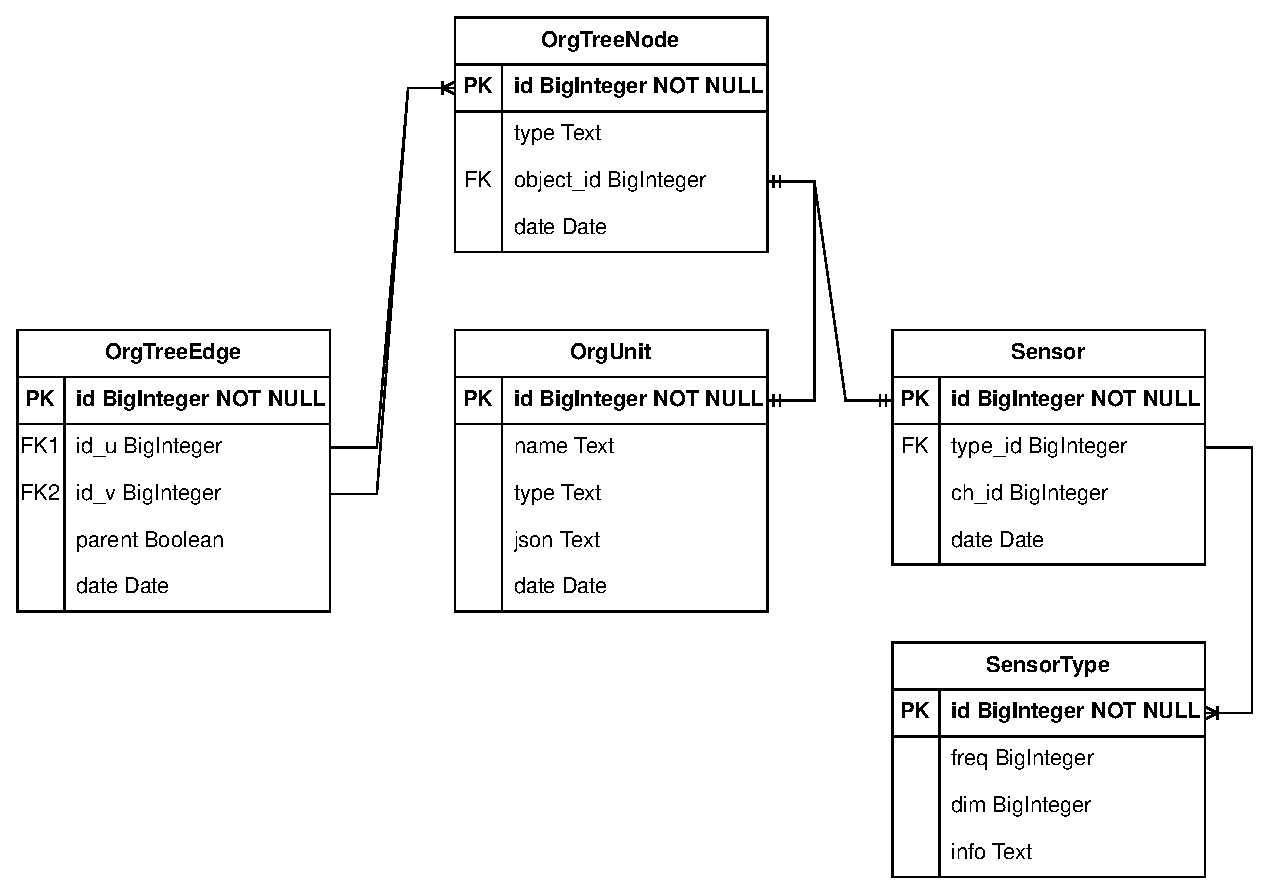
\includegraphics[scale=0.75]{../img/pg.drawio.eps}
  \caption{Модель организационной структуры}
  \label{datamodel}
\end{figure}

Основные способы управления временными рядами и деревом организационной структуры приведены на рисунке~\ref{usecases}.

\begin{figure}
  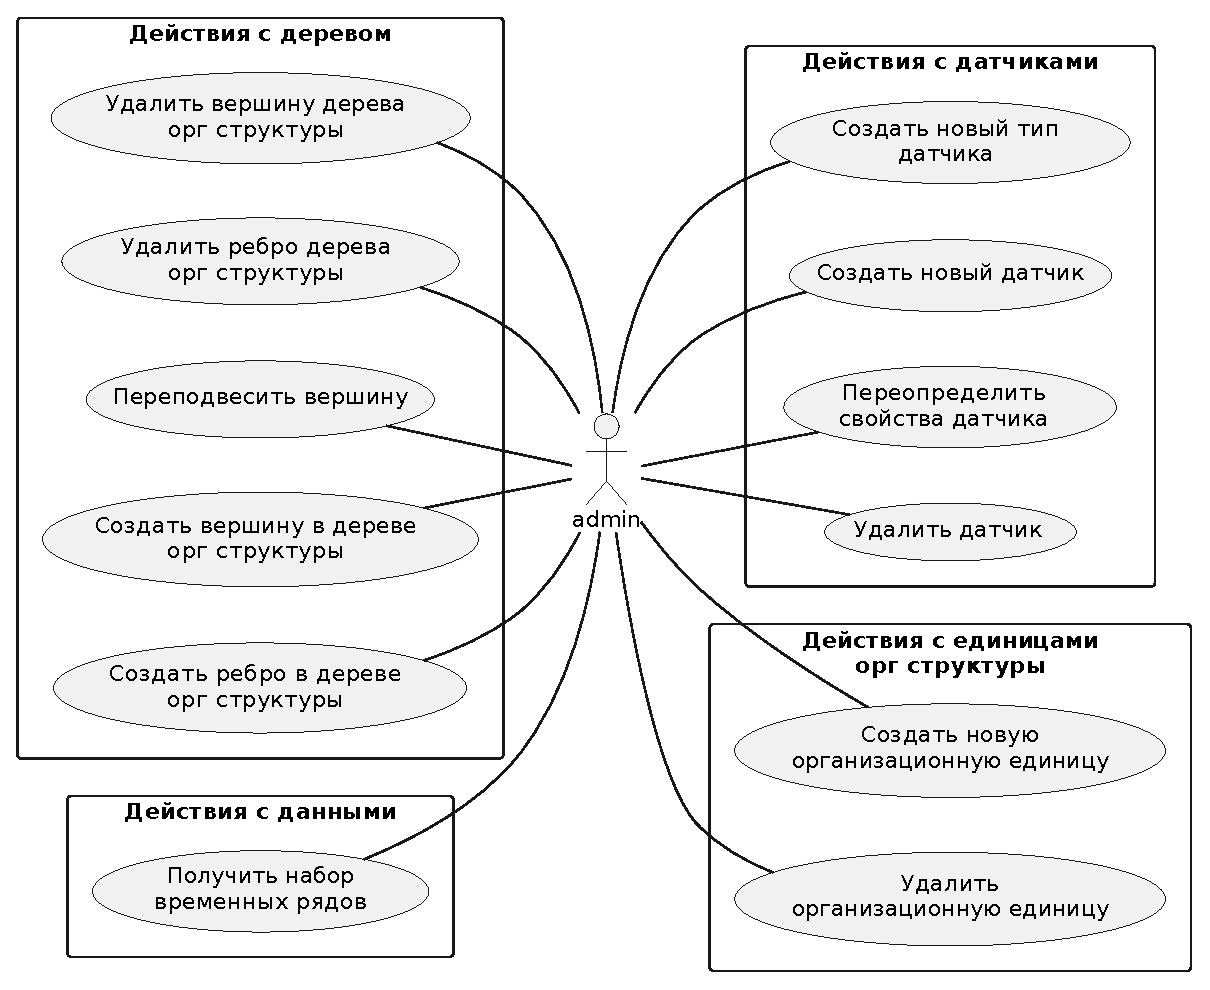
\includegraphics[scale=0.75]{../img/usecases.eps}
  \caption{Способы взаимодействия}
  \label{usecases}
\end{figure}

OrgTreeNode --- вершина графа организацонной структуры. Хранит уникальный идентификатор вершины, тип объекта (сенсор или единица организационной структуры) и его номер.

OrgTreeEdge --- ребро графа организационной структуры. id\_u и id\_v хранят начальную и конечную вершины ребра. parent указывает, является ли ребро от родителя к рёбенку или нет.  Уникальный идентификатор id нужен для реализации получения обратного ребра.

OrgUnit описывает единицу организационной структуры, имеет свой уникальный идентификатор. Поля name, type, json используются для хранения информации об единице и могут быть изменены при необходимости.

SensorType описывает тип датчика --- его частоту дискретизации и размерность данных, которые регистрирует датчик. info хранит служебную информацию о типе. Уникальный идентификатор id используется, чтобы задать тип определённому сенсору.

Sensor описывает датчик, так же имеет свой уникальный идентификатор. type\_id хранит идентификатор типа датчика, описанный выше. ch\_id содержит номер таблицы, в которой хранятся данные, регистрируемые датчиком.

Поля date обозначают, когда был удалён объект организационной структуры. Если объект не удалён, оно будет пустым. Это поле позволяет реализовать историю всех объектов организационной структуры, добавляя к модели персистентность.

Чтобы создать новый сенсор, нужно узнать, добавлен ли тип сенсора, затем добавить новый сенсор, создав под него новую таблицу. Добавление новой организационной единицы не требует никаких проверок.

Для создания вершнины дерева требуется определить, будет ли вершина соответствовать организационной еденице или датчику. Затем проверить, что соответствующая единица или датчик существуют на момент создания вершины.

При создании ребра между двумя вершинам выполняется проверка, что такое ребро не существует, чтобы избежать добавления кратных рёбер. Так же проверяем, что ребро не является петлёй. Добавляем два ребра --- прямое ребро $(u, v)$ с номером $id$ и истинным флагом $parent$, обратное $(v, u)$ с номером $id + 1$. Такое хранение рёбер позволяет получать обратное ребро. Допустим, без потери общности, индексация рёбер начинается с нуля. Если это не так, то при вычислении вычтем единицу. Пусть ребро $(u, v)$ имеет идентификатор $id$, тогда обратное ему ребро --- $id - 1$ либо $id + 1$. Если $(u, v)$ --- прямое ребро, то $id$ чётное или ноль, обратное ему --- $id + 1$, что так же равно $id \oplus 1$. Если $(u, v)$ --- обратное ребро, то $id$ нечётное, обратное ребро имеет номер $id - 1$, что опять же равно $id \oplus 1$, так как младший бит в $id$ равен единице, после применения операции побитового исключающего ИЛИ~\cite{XOR} с единицей станет нулём. Таким образом для получения обратного ребра необходимо выполнить побитовое исключающее ИЛИ номера ребра с единицей.

Удаление единицы организационной структуры или датчика осуществляется изменением поля $date$ на сегодня. Для удаления ребра найдём номер ребра и пометим его сегодняшней датой. То же самое сделаем и для обратного ребра, которое получим по принципу, описанному выше.

Для удаления вершины $u$ найдём её номер и номер ребра в родителя, пометим их сегодняшним числом. Теперь нужно каскадно удалить всё поддерево с корнем в этой вершине. Сформируем список смежности~\cite{graphs} вершины, используя таблицу с рёбрами дерева. Необходимо удалять только детей вершины $u$, поэтому выбираем рёбра с истинным флагом $parent$. Выполним обход в глубину~\cite{dfs1, dfs2} из вершины $u$ по этим рёбрам, вызывая функцию удаления. Обход в глубину имеет сложность $O(n + m)$, где $n$ --- количество вершин в поддереве, $m$ --- количество рёбер. Так как корневое поддерево~\cite{rooted-trees} сохраняет свойства дерева, $m = n - 1$, поэтому сложность $O(n)$.

Для переподвешивания вершины нужно сперва удалить ребро, соединяющее её с родителем, а затем добавить новое ребро.

Для визуализации дерева организационной структуры в реальном времени достаточно выбрать всё содержание таблиц, содержащих вершины и рёбра дерева. Удалённые элементы помечены какой-то датой, для выборки объектов, существующий на данных момент времени, следует выбирать записи, в которых поле $date$ пустое.

С помощью обхода в глубину так же осуществляется сбор данных с датчиков, находящихся в поддереве организационной единицы. Обход находит все таблицы датчиков и необходимые столбцы, после чего происходит выборка и интерполяция значений датчиков. Подробно объединение значений датчиков описано ниже.

\subsection{Стек используемых технологий}

Программный продукт реализован на языке программирования Python~\cite{Python}. Он имеет простой и понятный синтаксис. Динамическая типизация обеспечивает высокую скорость разработки. Большой набор стандартных библиотек позволяет решать широкий спекрт задач. С помощью встроенного менеджера пакетов pip возможно легко установливать сторонние библиотеки. Python является интерпретируемым языком программирования высокого уровня, обладает высокой кроссплатформенностью, достаточно установить интерпретатор языка и запустить модуль управления временными рядами. Python часто используется для анализа данных и машинного обучения, так как обладает мощными библиотеками. В работе используется NumPy~\cite{numpy}, который обладает инструментами для работы с временными рядами.

FastAPI~\cite{FastAPI} представляет собой веб-фреймворк для Python, позволяющий быстро создавать производительные веб-приложения. Для демоснтрации работы используется SwaggerUI~\cite{swaggerui}, который визуализирует и позволяет легко взаимодействовать с веб-интерфейсом. Обе технологии основаны на стандарте OpenAPI~\cite{OpenAPI}.

PostgreSQL --- реляционная система управления базами данных~\cite{postgresql}. Она хранит данные в виде таблиц, состоящих из строк и столбцов. Строка представляет собой отдельную запись, а столбец отдельное поле. Таблицы связаны между собой с помощью ключей. Это позволяет эффективно организовывать данные, а так легко извлекать информацию из нескольких таблиц.

PostgreSQL обеспечивает надёжное хранение данных и защиту от потери информации в случае сбоев. Граф организационной структуры предприятия небольшой, однако может менятся в ходе работы. PostgreSQL обладает достаточной гибкостью и высокой скоростью работы для добавления таблиц и полей.

ClickHouse --- столбцовая база данных, специализирующаяся на обработке больших объёмов информации в реальном времени~\cite{clickhouse}. Она отлично подходит для управления временными рядами, так как обеспечивает высокую скорость записи и чтения данных. Датчики на предприятии могут иметь высокую частоту опроса, поэтому важно уметь добавлять записи в реальном времени.

SQLAlchemy является библиотекой для работы с базами данных на основе объектно-ориентированного подхода~\cite{SQLAlchemy}. Она поддерживает множество систем управления базами данных, в том числе PostgreSQL~\cite{SQLAlchemy-pg} и ClickHouse~\cite{SQLAlchemy-ch}. Библиотека позволяет разработчикам создавать классы, которые соответствуют таблицам в базе данных. Эти классы могут быть использованы для выполнения запросов к базе данных, а также для создания, изменения и удаления записей.

Docker создаёт контейнеры под базы данных, тем самым изолирует их от других приложений и сервисов, повышая стабильность и безопасность~\cite{Docker}. Контейнер можно легко перенести из одной среды в другую и развернуть на любой операционной системе. Виртуальные машины потребляют гораздо больше ресурсов, чем контейнеры, поэтому Docker позволяет значительно сократить затраты на вычислительную инфраструктуру~\cite{Habr-VM}.

Для простого управления несколькими контейнерами используется Docker Compose~\cite{Docker-Compose}. Достаточно описать все контейнеры в одном YAML-файле и запустить их командой \texttt{docker-compose up}.

GraphViz позволяет визуализировать дерево организационной структуры~\cite{Graphviz}. Изображение создаётся в формате svg или png~\cite{Graphviz-formats} в реальном времени на основе данных выборки из таблиц с вершинами и рёбрами графа.

\subsection{Алгоритм управления временными рядами}

Каждый датчик имеет свою отдельную таблицу в ClickHouse, её номер хранится в поле ch\_id. При изменении типа датчика создаётся новая таблица~\cite{ch-create-table,ch-data-types}, чтобы не перестраивать старую и сохранить историю о предыдущих измерениях.

В работе данные генерируются синтетически для демонстрации работы программного продукта. Запрос генерации требует промежуток времени и номер вершины, для поддерева которого следует генерировать данные. С помощью обхода в глубину находятся все номера таблиц в ClickHouse для соответствующих датчиков, затем данные генерируются и вставляются в таблицы~\cite{ch-insert1,ch-insert2,ch-insert3,yield}.

Для хранения временных рядов используется таблица с движком MergeTree~\cite{ch-engines,ch-mergetree}. Эта структура данных похожа на Log-Structured Merge Tree, которое используется во многих СУБД. Данные хранятся в отсортированном виде по первичному ключу. Традиционные B-деревья имеют низкую производительность вставки большого количества элементов. LSM выполняет эту операцию быстрее за счёт накопления данных в буфере и последующего слияния с деревом на фоне.

Первичный ключ для временного ряда --- время. В таком случае замеры датчиков всегда хранятся в хронологическом порядке, и выборка данных выполняется быстрее, как показано в таблице~\ref{sample1}.

\begin{table}
  \caption{Пример хранения данных датчика в таблицу ClickHouse}
  \fontsize{12pt}{18pt}\selectfont
  \begin{tabular}{|c|c|c|c|}\hline
    \textbf{Time, ms}          & \textbf{Sensor\_3\_value\_1} & \textbf{Sensor\_3\_value\_2} & \textbf{Sensor\_3\_value\_3} \\ \hline
    2023-04-12 08:32:16.012345 & 100.0                        & 39.9                         & 10.0                         \\ \hline
    2023-04-12 08:32:16.512345 & 99.9                         & 40.1                         & 10.5                         \\ \hline
    2023-04-12 08:32:17.012345 & 100.0                        & 40.0                         & 11                           \\ \hline
  \end{tabular}
  \label{sample1}
\end{table}

Датчики могут иметь разные частоты дискретизации, то есть иметь актуальные замеры в разные моменты времени. Например, датчик с частотой дискретизации равной $2$ делает замеры в моменты времени $1$, $1.5$ и $2$ секунды, а датчик с частотой $3$ в моменты $1$, $1.333$, $1.667$ и $2$ секунды. Запрос выборки временных рядов датчиков подразумевает, что будут возвращены все значения датчиков в каждый момент времени, то есть в $1$, $1.333$, $1.5$, $1.667$ и $2$ секунды. Неизвестные значения датчиков должны быть интерполированы последними известными на данный момент времени данными, как показано в таблице~\ref{sample2}.

\begin{table}
  \caption{Пример интерполяции данных датчиков с разными частотами дискретизации}
  \fontsize{12pt}{18pt}\selectfont
  \begin{tabular}{|c|c|c|c|}\hline
    \textbf{Time, ms}       & \textbf{Sensor\_1\_value\_1} & \textbf{Sensor\_2\_value\_1} \\ \hline
    2023-04-12 08:32:01.000 & 10.0                         & 20.0                         \\ \hline
    2023-04-12 08:32:01.333 & 10.0                         & 20.333                       \\ \hline
    2023-04-12 08:32:01.500 & 10.5                         & 20.333                       \\ \hline
    2023-04-12 08:32:01.667 & 10.5                         & 20.667                       \\ \hline
    2023-04-12 08:32:02.000 & 11.0                         & 21.000                       \\ \hline
  \end{tabular}
  \label{sample2}
\end{table}

Рассмотрим алгоритм объединения таблиц датчиков с разными частотами дискретизации. Пусть количество сенсоров в поддереве запроса равно $m$, $f_i$ --- частота дискретизации $i$-го датчика, $d_i$ --- размерность данных $i$-го датчика, ${\Delta}t$ --- количество секунд в запросе выборки. Тогда количество строк в результирующей матрице --- ${\Delta}t \cdot \sum^{m}_{i=1}{f_i}$, а количество столбцов --- $\sum^{m}_{i=1}{d_i} + 1$, так как один столбец хранит время. Размер матрицы ${\Delta}t \cdot \sum^{m}_{i=1}{f_i} $ на $\sum^{m}_{i=1}{d_i}$ + 1, хранить всю матрицу в оперативной памяти дорого, поэтому будем писать каждую строку в файл.

Обход в глубину находит все датчики и их номера таблиц в ClickHouse в поддереве организационной единицы, формирует столбцы, из которых нужно сделать выборку. Чтобы получить все моменты времени, выполняется выборка первого столбца времени для каждого датчика. Полученные моменты времени сортируются, среди них выбираются уникальные~\cite{np-unique}. Массив времён состоит из отсортированных блоков, поэтому сортировка выполняется быстрее, чем на случайных данных. Однако в худшем случае сложность сортировки будет $O(n \cdot \log{n})$, где $n$ --- размер сортируемого массива. Датчики формируют ${\Delta}t \cdot \sum^{m}_{i=1}{f_i}$ моментов времени, поэтому массив имеет такой размер. Итоговая сложность сортировки $O({\Delta}t \cdot \sum^{m}_{i=1}{f_i} \cdot \log{({\Delta}t \cdot \sum^{m}_{i=1}{f_i})})$.

Выборка из таблицы в ClickHouse возвращает итерируемый объект, для формирования данных строки и интерполяции данных используется метод двух указателей~\cite{two-pointers}. По сути идея сортировки слиянием~\cite{mergesort} расширяется на несколько массивов. Пусть текущая строка содержит момент времени $t_j$, для каждого датчика будем итерироваться по объекту выборки, пока время в записи не будет больше $t_j$, сохраняя предыдущую запись. Именно эта запись будет отвечать за значения датчика в момент времени $t_j$. Так как данные в таблице отсортированы по возрастанию времени, мы всегда будем находить последнее известное значение параметров на момент времени $t_j$. После этого можно заполненить строку таблицы соответствующими значениями с датчиков.

Так за один проход получается сформировать все значения датчиков для каждого момента времени. Объект выборки $i$-го датчика содержит ${\Delta}t \cdot f_i$ записей, поэтому сложность прохода по значениям одного датчика $O({\Delta}t \cdot f_i \cdot d_i)$. Сложность формирования одной строки $O(\sum^{m}_{i=1}{d_i})$. Формирование всей результирующей матрицы с учётом итерации по данным датчиков $O({\Delta}t \cdot \sum^{m}_{i=1}{f_i} \cdot \sum^{m}_{i=1}{d_i} + {\Delta}t \cdot \sum^{m}_{i=1}{(f_i \cdot d_i)})$. Так как ранее была выполнена сортировка массива времени, итоговая сложность ответа на запрос выборки временных рядов датчиков с разными частотами дискретизации $O({\Delta}t \cdot \sum^{m}_{i=1}{f_i} \cdot [\log({\Delta}t \cdot \sum^{m}_{i=1}{f_i}) + \sum^{m}_{i=1}{d_i}] + {\Delta}t \cdot \sum^{m}_{i=1}{(f_i \cdot d_i)})$. Пространственная сложность алгоритма $O({\Delta}t \cdot \sum^{m}_{i=1}{f_i} + \sum^{m}_{i=1}{d_i})$.

Для добавления новых данных достаточно вставить их в имеющиеся таблицы. Эта операция не требует перестроения структуры таблиц. Ещё один способ организации данных --- хранение данных всех датчиков в единой таблице. В таком случае запрос выборки не требует дополнительных вычислений, однако вставка затрудняется и требует перестроения таблицы. Для сравнения этого варианта с идеей хранить таблицу для каждого сенсора реализовано построение большой таблицы с генерацией данных по алгоритму, похожему на описанный для выборки выше. В следующей главе будет приведено сравнение производительности обоих вариантов.

\subsection{Исходный код модуля}

SQLAlchemy позволяет задавать структуру таблицы на основе объектно-ориентированного подхода, как показано на рисунке~\ref{src1}. Необходимо унаследовать класс от базового \texttt{declarative\_base()} и задать типы столбцов таблицы в соответствии с документацией~\cite{SQLAlchemy-data-types}, указать первичный ключ. Взаимодействие с модулем осуществляется с помощью json, поэтому необходимо преобразовывать объекты. Например, функция \texttt{Sensor\_to\_schema} преобразует объект класса \texttt{Sensor} в json.

\begin{figure}
  \fontsize{12pt}{14pt}\selectfont
  \lstinputlisting[language=Python]{src/1.py}
  \caption{Фрагмент кода для ребра дерева}
  \label{src1}
\end{figure}

Обход в глубину реализован с помощью рекурсии, как показано на рисунке~\ref{src4}. Функция сохраняет все сенсоры поддерева в словарь \texttt{dct\_Sensors} вместе с их типами. Это нужно для удобного последующего получения данных из таблиц датчиков. Чтобы получить список смежности вершины, используется функция, изображенная на рисунке~\ref{src5}. В ней выполняется два запроса к базе данных для получения ребра в родителя и ребёр в сыновей.

\begin{figure}
  \fontsize{12pt}{14pt}\selectfont
  \lstinputlisting[language=Python]{src/4.py}
  \caption{Фрагмент кода для обхода в глубину}
  \label{src4}
\end{figure}

\begin{figure}
  \fontsize{12pt}{14pt}\selectfont
  \lstinputlisting[language=Python]{src/5.py}
  \caption{Фрагмент кода для получения смежных вершин}
  \label{src5}
\end{figure}

При создании таблицы в ClickHouse необходимо учесть размеронсть данных, собираемых датчиком. Он может собирать сразу несколько показателей, поэтому нужно создать несколько столбцов. Декларативный подход позволяет сразу определить структуру таблицу, однако в случае с датчиками она неизвестна заранее, поэтому модуль формирует SQL-запрос к СУБД, как изображено на рисунке~\ref{src2}. В запросе указан движок таблицы и первичный ключ.
\begin{figure}
  \fontsize{12pt}{14pt}\selectfont
  \lstinputlisting[language=Python]{src/2.py}
  \caption{Фрагмент кода для создания таблицы датчика}
  \label{src2}
\end{figure}

Рассмотрим метод, реализующий взаимодействие с базами данных. На рисунке~\ref{src3} приведён метод добавления ребра дерева. Он принимает запрос и подключается к PostgreSQL. Выполняется проверка на петлю, затем проверка, что указанные в запросы вершины дерева сущетвуют и проверка, что ребро не было добавление ранее. Как было описано выше, в таблицу заносятся два ребра --- прямое и обратное. При возникновении ошибки следует возвращать исключение \texttt{HTTPException}~\cite{FastAPI-error}, соответствующее документации в SwaggerUI.

\begin{figure}
  \fontsize{12pt}{14pt}\selectfont
  \lstinputlisting[language=Python]{src/3.py}
  \caption{Фрагмент кода для добавления ребра дерева}
  \label{src3}
\end{figure}
